\chapter{Resultados}
\label{ch:Resultados}
\section{Resultados parciais}
\section{Abstrair o problema no contexto}
O contexto geral do trabalho é projetar e construir um sistema AM para auxiliar no diagnóstico da doença de Parkinson, utilizando sinais obtidos por dispositivos sEMG, e o problema principal gira em torno de como esse sistema será desenvolvido. Por se tratar da construção de um software, isso necessita de um planejamento prévio de como será feita essa construção, levando em consideração um conjunto de variáveis para tomada de decisões. Neste trabalho o sistema a ser desenvolvido se trata de um sistema AM, que requer uma maior atenção sobre algumas variáveis, como quantidade de recursos e tipos de dados obtidos, sendo que essas variáveis servem como indicadores para auxiliar a decisão de qual algoritmo utilizar para se encontrar a melhor solução possível para esse problema.

\section{Prova de conceito}
Para verificar a viabilidade do projeto, além de buscar entender o funcionamento da biblioteca \textit{scikit-learn}. Realizou-se uma prova de conceito, desenvolvendo um algoritmo utilizando o SVM, para predizer os dados relacionados a uma porta lógica XOR. Foram utilizados também o \textit{numpy} para as manipulações matemáticas e o \textit{matplotlib} para plotar o gráfico.

Como observado na Figura \ref{svmxor} na página \pageref{svmxor}, o svm conseguiu separar corretamente a maioria dos dados, sendo que, na imagem as bolas laranjas equivalem ao valor esperado '1', e as bolas azuis equivalem ao valor esperado '0'. Já os contornos equivalem ao valor atingido pelo SVM, ou seja, as bolas dentro da área azul foram preditas como '0' e  a bolas na área laranjada foram preditas como '1'.

\begin{figure}[!htb]
	\centering
	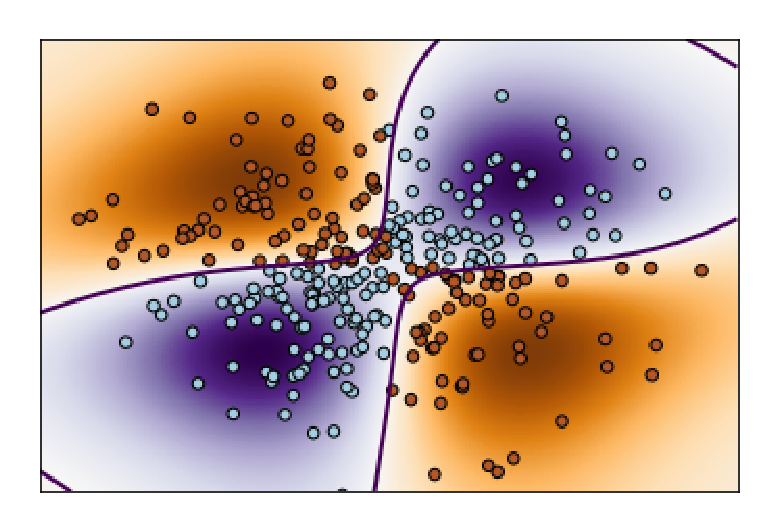
\includegraphics[width=0.8\textwidth]{figuras/xor.eps}
	\caption{SVM com a porta XOR.}
	\label{svmxor}
\end{figure}